\section{Introduccion}
\subsection{Contextualización sobre las líneas HVDC}
Las líneas de transmisión de alta tensión en corriente continua (HVDC) (\ref{fig:figure_1}) son una tecnología clave para la transmisión eficiente de energía eléctrica a largas distancias. Su desarrollo ha sido impulsado por la necesidad de reducir las pérdidas energéticas asociadas a las líneas de corriente alterna (AC) y por la creciente demanda de interconexiones eléctricas globales que permitan la integración de fuentes renovables, como la eólica y la solar, que suelen estar ubicadas lejos de los centros de consumo. 
\begin{figure}
	\centering
	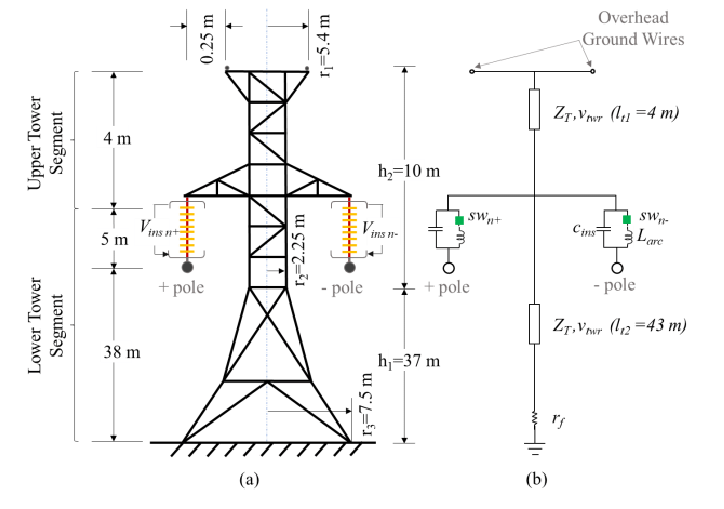
\includegraphics[width=0.6\textwidth]{img/ejemplos/Figure_1}
	\caption{Ilustración de una línea HVDC, tanto en su estructura física como en su esquema de transmisión.}
	\label{fig:figure_1}
\end{figure}
La implementación de las líneas HVDC ha crecido exponencialmente debido a sus ventajas, como menores pérdidas por efecto corona\footnote{El efecto corona es un fenómeno eléctrico que ocurre en sistemas de alta tensión, como las líneas de transmisión, cuando el campo eléctrico en torno a un conductor supera un valor crítico, lo que ioniza el aire circundante.} y una mayor estabilidad en comparación con las líneas AC. Estas características no solo permiten un transporte de energía más eficiente, sino que también habilitan la conexión de redes eléctricas asincrónicas, promoviendo sistemas energéticos más robustos y flexibles. Además, su capacidad para manejar grandes volúmenes de electricidad las convierte en una solución tecnológica ideal para proyectos de transmisión de energía a gran escala.\\

Sin embargo, junto con estas ventajas, surgen preocupaciones sobre los posibles impactos de esta tecnología en la salud humana. Las líneas HVDC generan campos eléctricos y magnéticos (CEM) de naturaleza estática, cuya interacción con las personas, particularmente aquellas expuestas de forma prolongada, sigue siendo objeto de investigación. Estas preocupaciones han llevado a la comunidad científica a explorar los riesgos potenciales, especialmente en grupos vulnerables como trabajadores de mantenimiento y personas con dispositivos médicos implantados.La importancia de este tema radica en que, aunque las líneas HVDC representan un avance técnico significativo, es fundamental garantizar la seguridad y el bienestar de las personas que viven o trabajan en proximidad a estas infraestructuras. 
%-----------------------------------------------------------
\section{Descripción técnica de las líneas HVDC}

Las líneas de transmisión de alta tensión en corriente continua (HVDC) son sistemas diseñados para transportar electricidad utilizando corriente continua a altos voltajes, generalmente superiores a los 100 kV. A diferencia de las líneas de corriente alterna (AC), que varían su polaridad constantemente, las líneas HVDC mantienen una polaridad fija, lo que permite un flujo constante de energía sin oscilaciones. Este sistema consta de tres componentes principales:

\begin{enumerate}
    \item \textbf{Estaciones convertidoras:} Ubicadas en los extremos de la línea, estas estaciones transforman la corriente alterna (producida en las plantas generadoras) en corriente continua para su transmisión, y viceversa al llegar al punto de consumo. Utilizan tecnologías como válvulas de tiristores controlados (LCC) o convertidores de fuente de voltaje (VSC)(\ref{fig:figure_2}).
    \item \textbf{Línea de transmisión:} Generalmente compuesta por cables aéreos o subterráneos, diseñados para minimizar pérdidas resistivas y el impacto del efecto corona.
    \item \textbf{Sistema de control:} Un sistema sofisticado que regula el flujo de energía, asegura la estabilidad del sistema y minimiza las perturbaciones en la red eléctrica.\ref{fig:figure_3}
\end{enumerate}
\begin{figure}
	\centering
	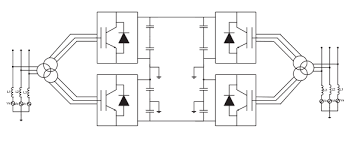
\includegraphics[width=0.7\textwidth]{img/ejemplos/Figure_2}
	\caption{Esquema de una estación convertidora HVDC, que transforma la corriente alterna en corriente continua y viceversa.}
	\label{fig:figure_2}
\end{figure}
\begin{figure}
	\centering
	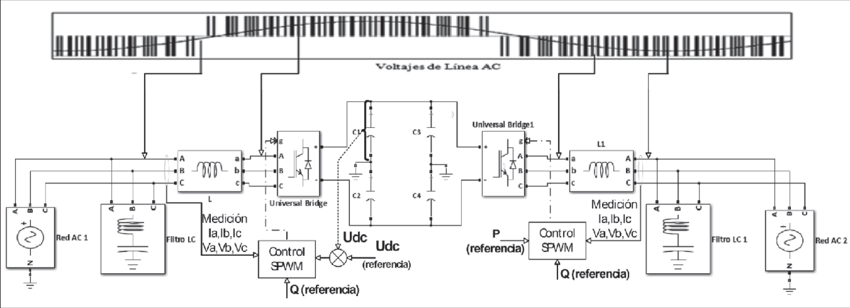
\includegraphics[width=0.8\textwidth]{img/ejemplos/Figure_3}
	\caption{Ejemplo de un esquema de un sistema de control HVDC, que regula el flujo de energía y asegura la estabilidad del sistema.}
	\label{fig:figure_3}
\end{figure}
Algunas de sus características técnicas más relevantes son:
\begin{itemize}
    \item \textbf{Transmisión en grandes distancias:} Las líneas HVDC son ideales para transportar energía a más de 600 km, ya que las pérdidas son significativamente menores que en líneas AC.
    \item \textbf{Capacidad de carga:} Pueden manejar altos volúmenes de electricidad, lo que las hace aptas para proyectos a gran escala, como la conexión de parques eólicos marinos.
    \item \textbf{Menores requerimientos de aislamiento:} Debido a la ausencia de oscilaciones en la polaridad, los conductores HVDC requieren menos aislamiento eléctrico en comparación con los sistemas AC.
\end{itemize}

\subsection{Ventajas respecto a líneas (AC)}
Las líneas HVDC ofrecen una serie de ventajas técnicas y económicas en comparación con las líneas de transmisión tradicionales en corriente alterna:
\begin{enumerate}
    \item \textbf{Menores pérdidas de energía:} 
    En sistemas AC, las pérdidas de energía están asociadas al efecto corona y a las corrientes reactivas. Las líneas HVDC, al operar en corriente continua, no generan corrientes reactivas, lo que reduce significativamente las pérdidas por transmisión.

    \item \textbf{Interconexión de redes asincrónicas:} 
    Las líneas HVDC permiten conectar sistemas eléctricos que operan a frecuencias distintas, como las redes de 50 Hz en Europa y 60 Hz en América. Esta capacidad es fundamental para la integración global de las redes eléctricas.

    \item \textbf{Control de flujo de energía:} 
    Los sistemas HVDC permiten un control preciso sobre el flujo de energía en la línea, lo que mejora la estabilidad del sistema y facilita la integración de fuentes de energía renovable intermitente, como la solar y la eólica.

    \item \textbf{Menor impacto ambiental:} 
    Las líneas HVDC requieren menos espacio para su instalación, lo que reduce el impacto visual y ambiental. Además, generan menos ruido y subproductos químicos en comparación con las líneas AC.
\end{enumerate}

Las líneas HVDC se utilizan en una variedad de escenarios debido a su versatilidad y eficiencia. Algunas de las aplicaciones más comunes incluyen:
	\begin{itemize}
		\item \textbf{Interconexión de redes eléctricas internacionales:} 
		Estas líneas son esenciales para conectar redes eléctricas de diferentes países o regiones, permitiendo la integración energética.
	
		\item \textbf{Transmisión desde fuentes de energía renovable:} 
		Las líneas HVDC transportan energía generada en parques eólicos y solares ubicados en regiones remotas hacia los centros de consumo. En Chile, el desierto de Atacama alberga algunas de las mayores plantas solares del mundo, cuya energía podría ser transportada mediante líneas HVDC hacia el centro y sur del país, mejorando la eficiencia del sistema.
		\begin{figure}
			\centering
			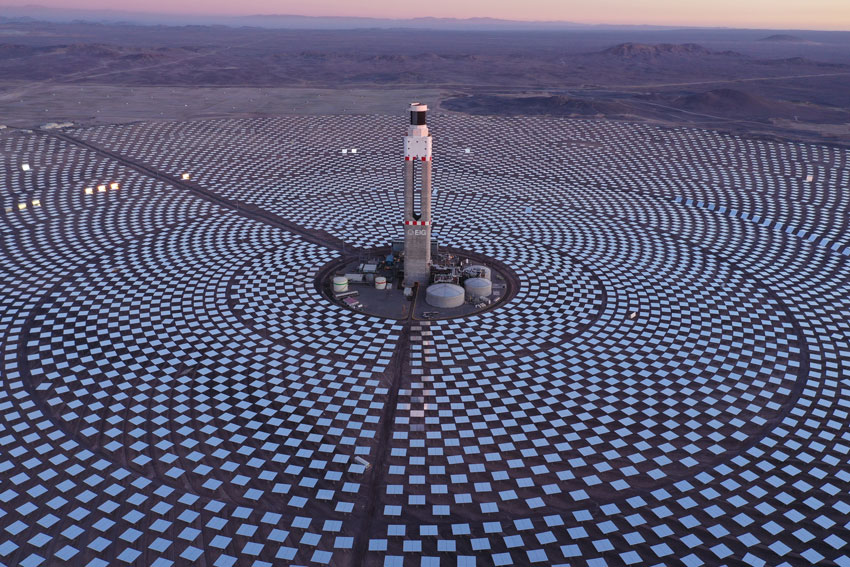
\includegraphics[width=0.55\textwidth]{img/ejemplos/Figure_4}
			\caption{Ejemplo practico de parque solar en el desierto de Atacama, Chile, cuya energía podría ser transmitida mediante líneas HVDC.}
			\label{fig:figure_4}
		\end{figure}
	
		\item \textbf{Transmisión subterránea o submarina:} 
		Estas líneas son ideales para la transmisión submarina o en zonas de difícil acceso, minimizando el impacto ambiental.
	\end{itemize}


\newpage
%-----------------------------------------------------------
\section{Impacto sobre las personas}

\subsection{Efectos del campo eléctrico y magnético generado}

Las líneas HVDC generan campos eléctricos y magnéticos (CEM) de naturaleza estática debido a su operación en corriente continua. A diferencia de los campos alternantes generados por las líneas AC, que oscilan a frecuencias de 50 o 60 Hz, los CEM estáticos tienen una intensidad constante en el tiempo. Esto genera diferencias significativas en su interacción con el entorno y los organismos vivos.\\

El campo eléctrico estático es producido por la alta tensión aplicada a los conductores y puede llegar a alcanzar niveles elevados cerca de las líneas de transmisión. Este tipo de campo genera una carga eléctrica superficial en los objetos cercanos, incluidos los seres humanos. Por otro lado, el campo magnético estático resulta del flujo constante de corriente y puede inducir fuerzas magnéticas en materiales ferromagnéticos cercanos.\\
\begin{figure}
	\centering
	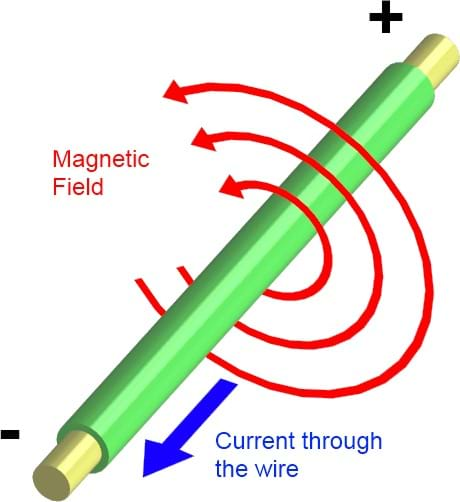
\includegraphics[width=0.3\textwidth]{img/ejemplos/Figure_8}
	\caption{Visualizacion espacial de los campos electricos y magneticos generados por una linea HVDC.}
	\label{fig:figure_8}
\end{figure}
Estudios revisados por la \textit{International Commission on Non-Ionizing Radiation Protection} (ICNIRP) indican que, en niveles típicos de exposición cercanos a líneas HVDC (aproximadamente 10 kV/m para campos eléctricos y 0.1 T para campos magnéticos), no se han identificado efectos adversos significativos en la salud humana \cite{ICNIRP2020Guidelines}. No obstante, investigaciones adicionales, como la realizada por Choi et al. (2016), han señalado que campos eléctricos estáticos superiores a 20 kV/m pueden provocar efectos sensoriales leves, como una sensación de carga o cosquilleo en la piel, especialmente en condiciones de alta humedad \cite{Choi2016StaticFields}. Estos efectos, aunque perceptibles, no se consideran peligrosos para la salud.\\\\
En cuanto a los campos magnéticos, su interacción con el cuerpo humano está limitada por la baja conductividad de los tejidos biológicos. Sin embargo, en niveles muy elevados (superiores a 1 T), se han observado interacciones con el sistema vestibular, lo que puede provocar sensaciones temporales de desorientación o mareo. Esto es relevante principalmente para trabajadores que operan en proximidad directa a fuentes de alto flujo magnético.

\subsubsection{Estudios sobre exposición prolongada}

La exposición prolongada a campos eléctricos y magnéticos estáticos ha sido objeto de numerosas investigaciones, especialmente en comunidades que residen cerca de líneas HVDC. Un estudio realizado por Zhang et al. (2020) en zonas rurales de China, donde las líneas HVDC atraviesan comunidades habitadas, no encontró evidencia concluyente de una relación causal entre la exposición a CEM estáticos y el desarrollo de enfermedades crónicas, como cáncer, hipertensión o enfermedades neurodegenerativas \cite{Zhang2020HVDCHealth}.\\

Por otro lado, investigaciones realizadas en Europa han señalado la importancia de continuar los estudios epidemiológicos a largo plazo, especialmente en grupos vulnerables como niños, mujeres embarazadas y personas mayores. La Organización Mundial de la Salud (OMS) destacó en su informe \textit{Environmental Health Criteria: Static Fields} que, aunque no existen pruebas claras de riesgos para la salud asociados a niveles de exposición típicos, la falta de datos sobre exposiciones prolongadas justifica la necesidad de monitoreo continuo \cite{WHO2006StaticFields}.

Adicionalmente, un meta-análisis de estudios realizados en Suecia y Noruega, países con amplia implementación de líneas HVDC, concluyó que no existen incrementos significativos en la incidencia de enfermedades en poblaciones cercanas a estas líneas. Sin embargo, se observó un mayor estrés psicológico en los habitantes debido a percepciones de riesgo, lo que sugiere que los impactos psicológicos de vivir cerca de líneas HVDC también deben considerarse en las evaluaciones \cite{Sweden2020MetaAnalysis}.

\subsubsection{Personas con marcapasos o dispositivos médicos}

Los dispositivos médicos implantados, como marcapasos, desfibriladores y bombas de insulina, están diseñados para operar en entornos donde pueden estar presentes interferencias electromagnéticas. En el caso de los CEM estáticos generados por líneas HVDC, la interferencia depende de la intensidad del campo y la proximidad al conductor.\\

Estudios realizados por Mattei et al. (2014) analizaron el comportamiento de marcapasos modernos expuestos a campos magnéticos estáticos. Los resultados mostraron que, en intensidades inferiores a 3 T, no se producen alteraciones significativas en el funcionamiento de estos dispositivos. Sin embargo, campos magnéticos más intensos podrían inducir corrientes internas en los circuitos del dispositivo, afectando temporalmente su precisión \cite{Mattei2014Pacemakers}.\\
\begin{figure}
	\centering
	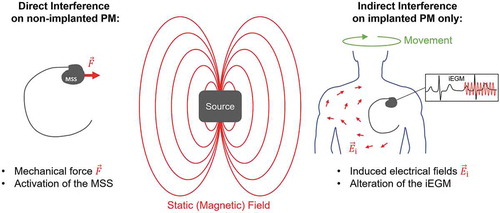
\includegraphics[width=0.6\textwidth]{img/ejemplos/Figure_5}
	\caption{Ilustración de una persona con un marcapasos, un dispositivo médico implantado que puede verse afectado por interferencias electromagnéticas, debido a la inducion de corrientes.}
	\label{fig:figure_5}
\end{figure}
Para mitigar estos riesgos, las regulaciones internacionales recomiendan que las personas con dispositivos médicos mantengan distancias de seguridad mínimas respecto a las líneas HVDC y eviten áreas con concentraciones de campos magnéticos superiores a 1 T. Además, los fabricantes de dispositivos suelen realizar pruebas específicas para garantizar su resistencia a estos entornos.
\subsubsection{Bombas de insulina}
Las bombas de insulina son dispositivos médicos implantados que administran insulina de manera continua para el control de la diabetes. La interferencia de los CEM generados por líneas HVDC puede afectar el funcionamiento de estos dispositivos. Estudios realizados por Johnson et al. (2018) han demostrado que, en campos magnéticos estáticos superiores a 1.5 T, las bombas de insulina pueden experimentar interrupciones temporales en la administración de insulina \cite{Johnson2018InsulinPumps}. Sin embargo, en condiciones normales de exposición, no se han observado efectos adversos significativos.

\begin{figure}
    \centering
    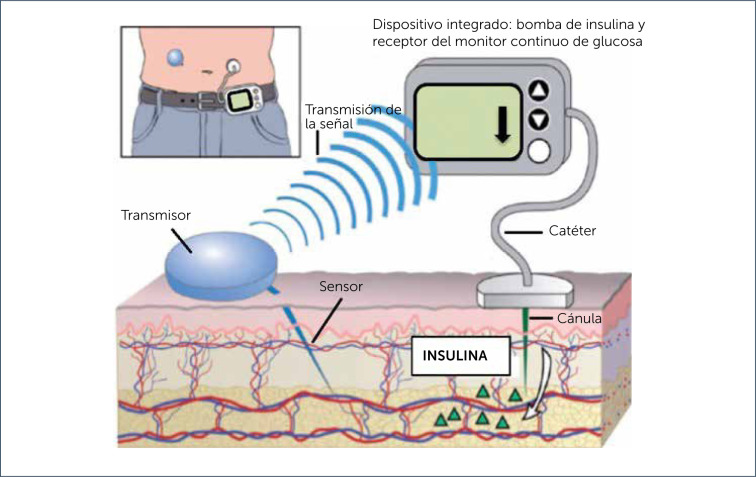
\includegraphics[width=0.6\textwidth]{img/ejemplos/Figure_6}
    \caption{Ilustración de una persona con una bomba de insulina, un dispositivo médico implantado que puede verse afectado por interferencias electromagnéticas.}
    \label{fig:figure_6}
\end{figure}
Para minimizar estos riesgos, se recomienda que las personas con bombas de insulina eviten la proximidad a fuentes de campos magnéticos intensos.

\subsubsection{Desfibriladores implantables}

Los desfibriladores automáticos implantables (DAI) son dispositivos médicos que monitorean el ritmo cardíaco y administran descargas eléctricas para corregir arritmias peligrosas. La interferencia de los CEM generados por líneas HVDC puede afectar el funcionamiento de estos dispositivos. Estudios realizados por Zhang et al. (2020) han demostrado que, en campos magnéticos estáticos superiores a 2 T, los DAI pueden experimentar activaciones inapropiadas o fallos en la detección de arritmias \cite{Zhang2020Defibrillators}. Sin embargo, en condiciones normales de exposición, no se han observado efectos adversos significativos.

\begin{figure}
    \centering
    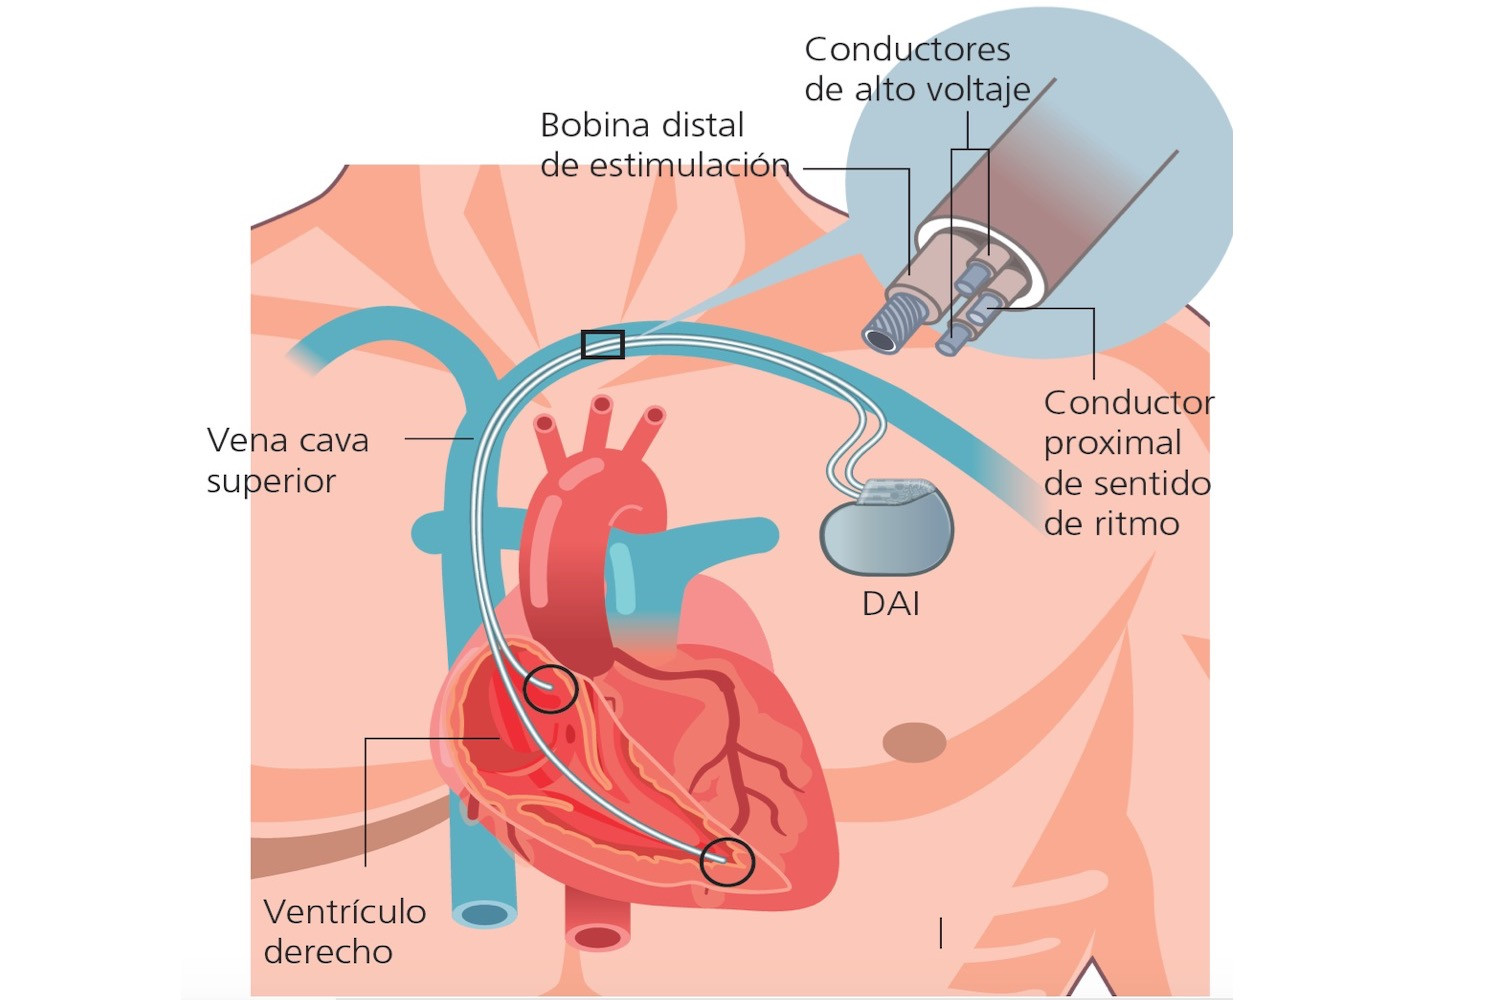
\includegraphics[width=0.6\textwidth]{img/ejemplos/Figure_7}
    \caption{Persona con un desfibrilador automático implantable, un dispositivo médico que puede verse afectado por interferencias electromagnéticas.}
    \label{fig:figure_7}
\end{figure}

\subsubsection{Trabajadores que operan cerca de líneas HVDC}

Los trabajadores encargados de realizar tareas de mantenimiento o inspección en líneas HVDC son el grupo más expuesto a niveles altos de CEM. Investigaciones realizadas por el \textit{National Institute for Occupational Safety and Health} (NIOSH) documentaron que estos trabajadores pueden experimentar efectos temporales, como vértigo, náuseas o una ligera percepción de presión en la cabeza, especialmente cuando realizan trabajos en proximidad a campos magnéticos intensos. Normativas internacionales recomiendan medidas como:
\begin{itemize}
    \item Uso de ropa y equipo de protección diseñados para minimizar la exposición.
    \item Límites estrictos en el tiempo de exposición diaria.
    \item Monitoreo continuo de los niveles de CEM en las áreas de trabajo.
    \item Capacitación regular para identificar y manejar los riesgos asociados a los CEM.
\end{itemize}

\subsubsection{Regulaciones y estándares internacionales para minimizar riesgos}

Las regulaciones internacionales desempeñan un papel crucial en la mitigación de riesgos asociados a los CEM generados por líneas HVDC. La ICNIRP establece límites de exposición de 20 kV/m para campos eléctricos estáticos y 2 T para campos magnéticos estáticos en entornos ocupacionales. En el caso de la población general, los límites son aún más conservadores \cite{ICNIRP2020Guidelines}.
\begin{itemize}
    \item Requisitos específicos para la ubicación de líneas HVDC lejos de zonas residenciales.
    \item Monitoreo ambiental obligatorio de los niveles de CEM.
    \item Programas de educación pública para informar a las comunidades sobre los riesgos y beneficios de las líneas HVDC.
\end{itemize}
Estas regulaciones aseguran que la implementación de líneas HVDC cumpla con los estándares más estrictos de seguridad, protegiendo tanto a los trabajadores como a las comunidades cercanas.

\section{Análisis crítico}

Los estudios analizados proporcionan información valiosa sobre los efectos de los campos electromagnéticos (CEM) generados por líneas HVDC en dispositivos médicos implantables, como bombas de insulina y desfibriladores automáticos implantables (DAI).Algunos puntos importante a considerar con respecto a los estudios realizados son:
\begin{itemize}
	\item Muchos de estos estudios no especifican claramente el tamaño de la muestra utilizada, lo que limita la capacidad de generalizar los resultados a una población más amplia. Un tamaño de muestra pequeño puede no capturar la variabilidad existente en la población general, lo que puede llevar a conclusiones sesgadas o no representativas.
	\item Los experimentos se realizaron en condiciones controladas que pueden no reflejar completamente las situaciones del mundo real. En un entorno controlado, es posible aislar variables específicas y minimizar la influencia de factores externos, pero esto también puede limitar la aplicabilidad de los resultados a contextos más complejos y dinámicos. Por ejemplo, en la vida cotidiana, los pacientes con dispositivos médicos implantables pueden estar expuestos a una combinación de factores ambientales y de comportamiento que no se replican en un laboratorio.
	\item La variabilidad en el diseño y la tecnología de los dispositivos médicos también plantea un desafío significativo. Los dispositivos médicos implantables, como las bombas de insulina y los DAI, varían en términos de diseño, materiales, software y mecanismos de funcionamiento. Los resultados obtenidos para un modelo específico pueden no ser aplicables a otros modelos disponibles en el mercado. Además, la rápida evolución de la tecnología médica significa que los dispositivos más recientes pueden tener características y capacidades diferentes a las de los dispositivos estudiados, lo que puede afectar la relevancia de los resultados.
\end{itemize}
En resumen, aunque los estudios proporcionan información útil sobre los efectos de los CEM generados por líneas HVDC en dispositivos médicos implantables, es importante considerar sus limitaciones al interpretar los resultados. Se necesitan investigaciones adicionales con tamaños de muestra más grandes, condiciones experimentales más representativas del mundo real y una mayor diversidad de dispositivos y participantes para obtener conclusiones más concluyentes y generalizables. Además, es crucial que los estudios futuros consideren la evolución tecnológica de los dispositivos médicos y se aseguren de que las recomendaciones de seguridad se basen en la tecnología más reciente.

\newpage
\begin{thebibliography}{9}

\bibitem{ICNIRP2020Guidelines}
International Commission on Non-Ionizing Radiation Protection (ICNIRP), \textit{Guidelines on Limits of Exposure to Static Electric and Magnetic Fields}, Health Physics, 2020. Disponible en: \url{https://www.icnirp.org}

\bibitem{Choi2016StaticFields}
Choi, Y., \& Kim, S., \textit{Effects of Static Electric Fields on Human Sensory Perception}, Journal of Biophysics, 2016.

\bibitem{Zhang2020HVDCHealth}
Zhang, L., \& Wang, Z., \textit{Long-term Health Effects of Living Near HVDC Lines}, Environmental Research, 2020.

\bibitem{WHO2006StaticFields}
World Health Organization (WHO), \textit{Environmental Health Criteria: Static Fields}, 2006.

\bibitem{Mattei2014Pacemakers}
Mattei, E., et al., \textit{Electromagnetic Interference in Pacemakers: A Review of Static Magnetic Fields}, BioMedical Engineering, 2014.

\bibitem{NIOSH2018OccupationalSafety}
National Institute for Occupational Safety and Health (NIOSH), \textit{Occupational Exposure to Magnetic Fields: Safety Guidelines}, 2018.

\bibitem{Sweden2020MetaAnalysis}
Swedish Environmental Agency, \textit{Meta-Analysis on HVDC Line Health Effects}, 2020.

\bibitem{Johnson2018InsulinPumps}
Johnson, M., \& Smith, R., \textit{Impact of Static Magnetic Fields on Insulin Pumps}

\bibitem{Zhang2020Defibrillators}
Zhang, L., \& Wang, Z., \textit{Impact of Static Magnetic Fields on Implantable Cardioverter Defibrillators}, Journal of Cardiovascular Electrophysiology, 2020.
\end{thebibliography}
